\section{Produto e Arquitetura Física}

O produto combina robôs aéreos e uma estação terrestre móvel. Segundo relato técnico da Spectro Cloud de 2025, a estação concentra \acp{GPU} de alto desempenho, e cada robô utiliza ventosas para coleta e um cabo para energia e dados~\cite{reeuwijk2025}. Essa organização mantém o processamento intensivo no solo, reduzindo o hardware computacional transportado em voo.

\begin{figure}[!htb]
    \centering
    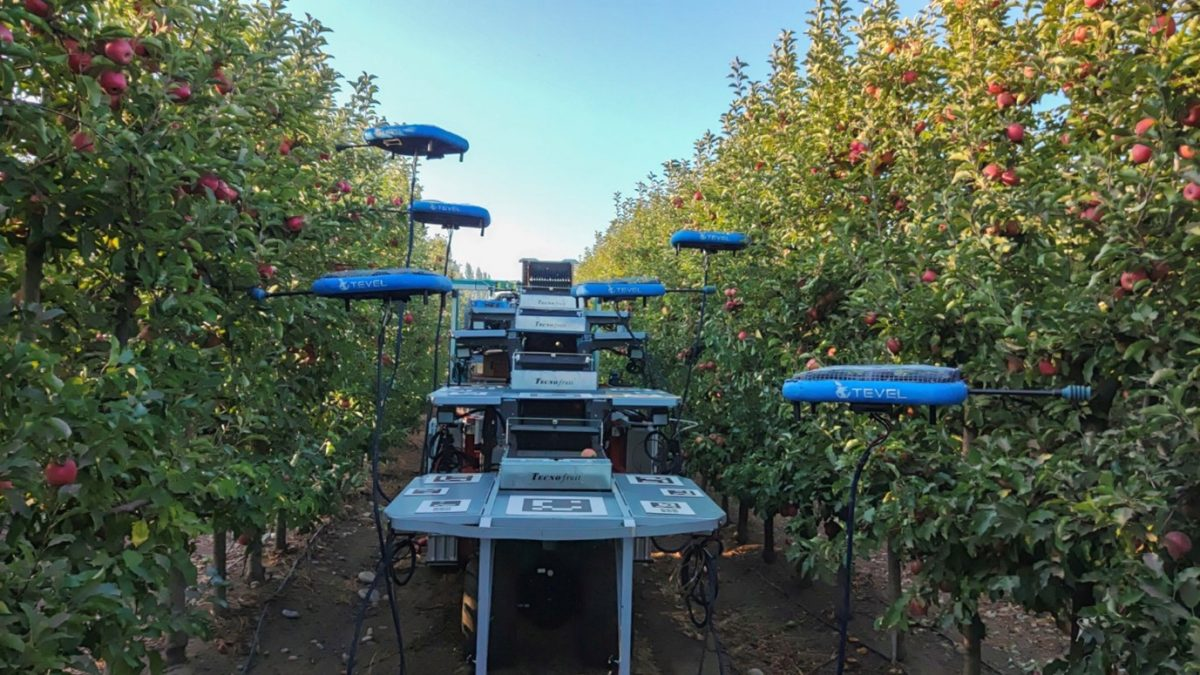
\includegraphics[width=0.98\linewidth]{figures/tevel_unufrutti.png}
    \caption{Robôs da Tevel em operação nos pomares da Unifrutti em Linares, Chile~\cite{unifrutti2023tevel}.}
    \label{fig:tevel_unifrutti}
\end{figure}

Na implantação chilena, oito \acp{FAR} foram integrados à plataforma de colheita da Darwin Harvesting Group, que recebia os frutos em recipientes~\cite{unifrutti2023tevel}. Essa quantidade caracteriza a implementação relatada, sem estabelecer uma configuração obrigatória para todas as versões.

A Tevel descreve detecção de frutos, folhagem e outros objetos, classificação por tamanho e maturação, rastreamento de frutos, fusão de dados, planejamento e execução de trajetórias e estabilização sob forças da folhagem e dos frutos~\cite{tevelTechnology}. Funcionalmente, a missão encadeia percepção, seleção do alvo, aproximação, desprendimento e entrega. A identificação correta do alvo não assegura acesso ou desprendimento adequados.

A publicação de patente WO2018033922A1 descreve navegação em malha fechada para aproximação e interação com frutos, mecanismos de coleta e estruturas de proteção entre folhas e galhos~\cite{maor2018harvesting}. Essas alternativas esclarecem a abordagem de engenharia, mas não comprovam a composição do produto comercial nem substituem os registros de operação que demonstram sua aplicação.

Como interpretação arquitetural, a autonomia resulta do conjunto aéreo-terrestre. A concentração de recursos no solo favorece o compartilhamento computacional e condiciona o desempenho à estação e aos enlaces locais. O compartilhamento de recursos e as restrições de movimento impostas pelos cabos devem ser considerados na adaptação ao pomar.